\subsection{Гистограммы и графики плотности распределения}
	\begin{figure}[H]
		\centering
		\begin{tabular}{ccc}
			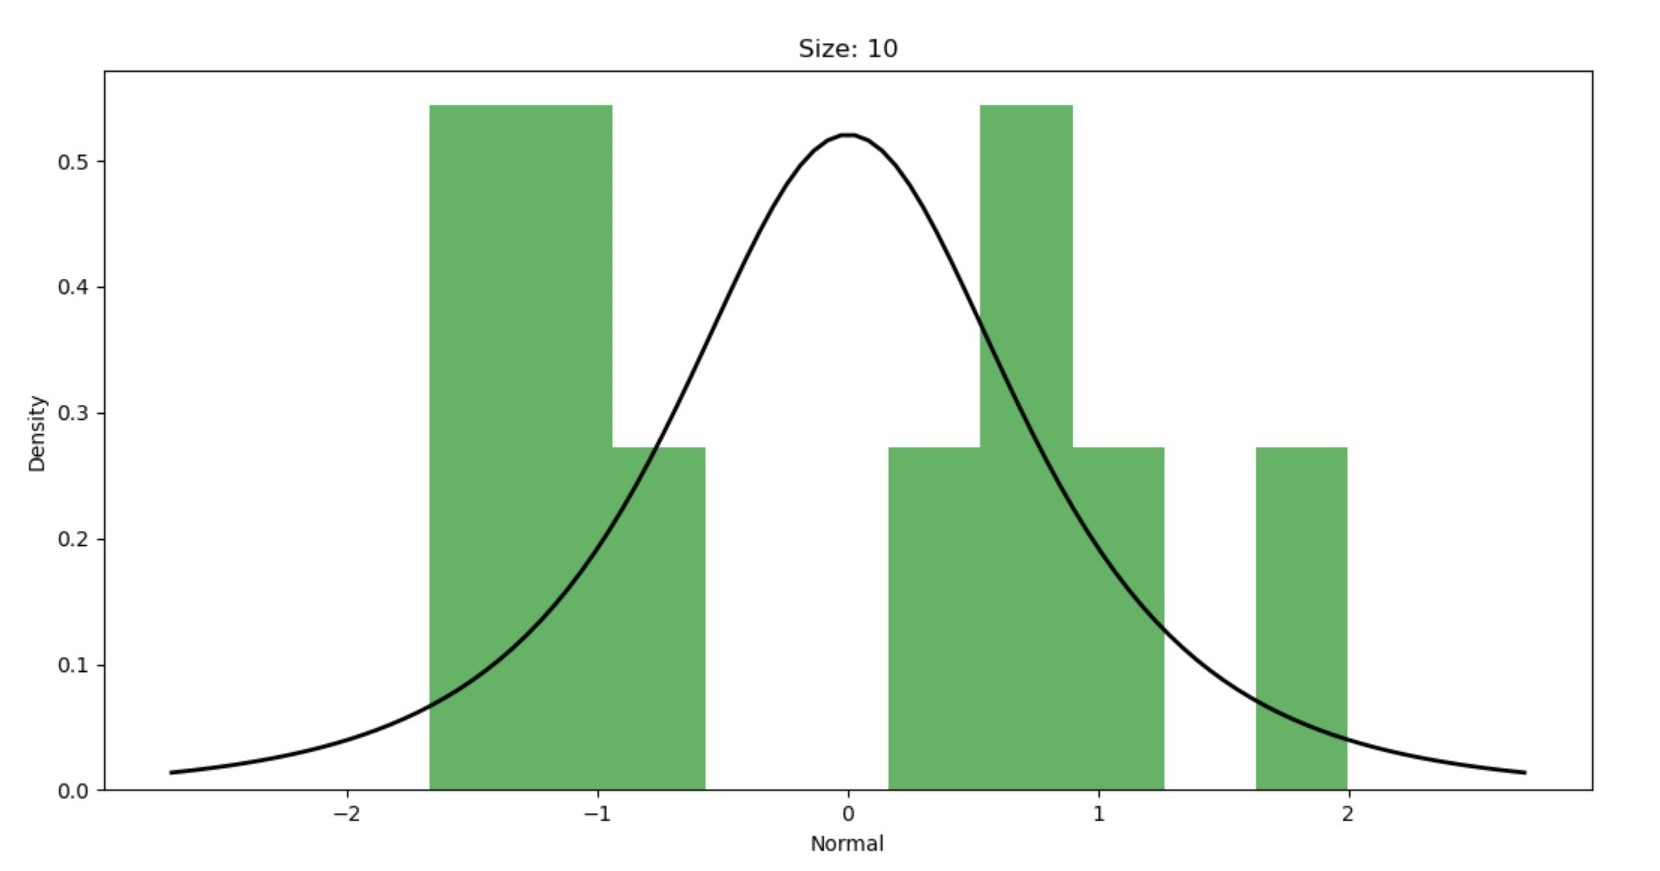
\includegraphics[width=55mm, height =0.25\textheight]{pics/n10.jpg}
			&
			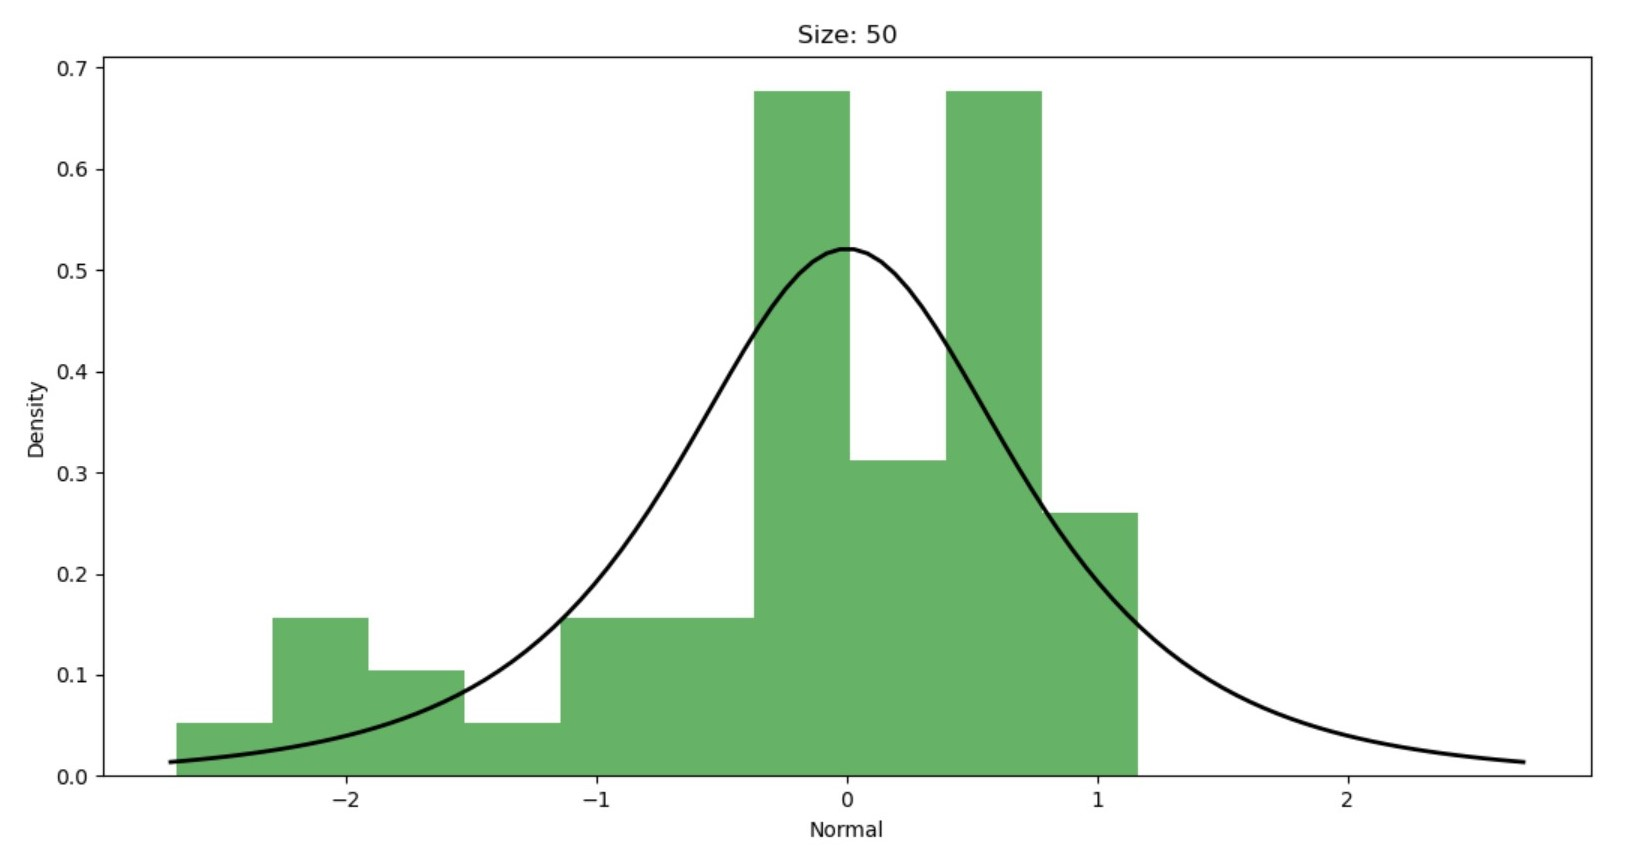
\includegraphics[width=55mm, height =0.25\textheight]{pics/n50.jpg}
			&
			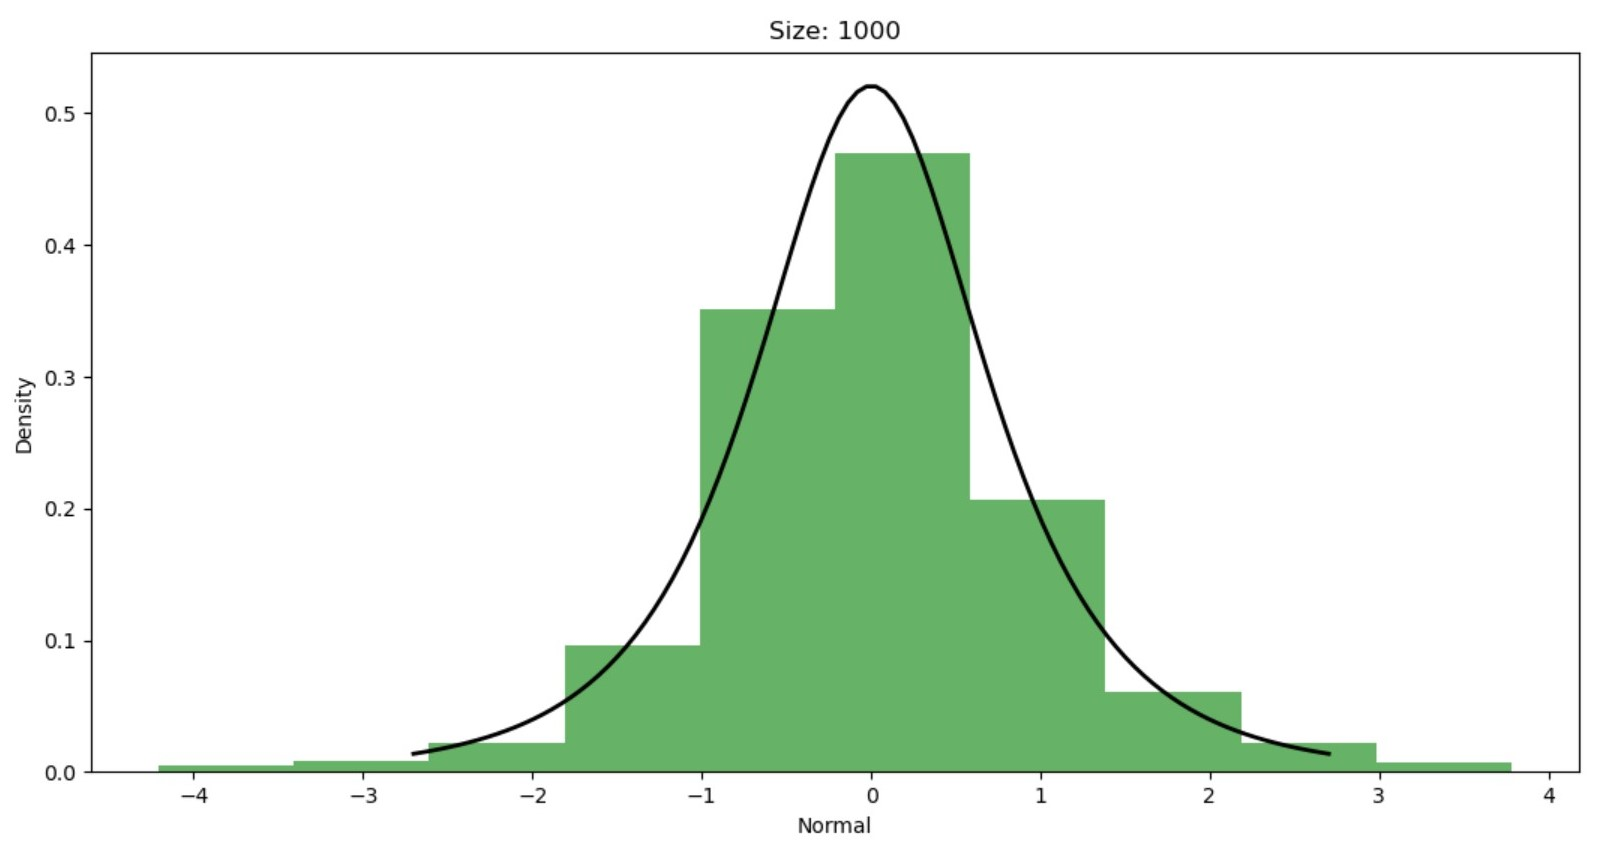
\includegraphics[width=55mm, height =0.25\textheight]{pics/n1000.jpg}
		\end{tabular}
		\caption{Нормальное распределение}
		\label{fig:normal}
	\end{figure}

	\begin{figure}[H]
		\centering
		\begin{tabular}{ccc}
			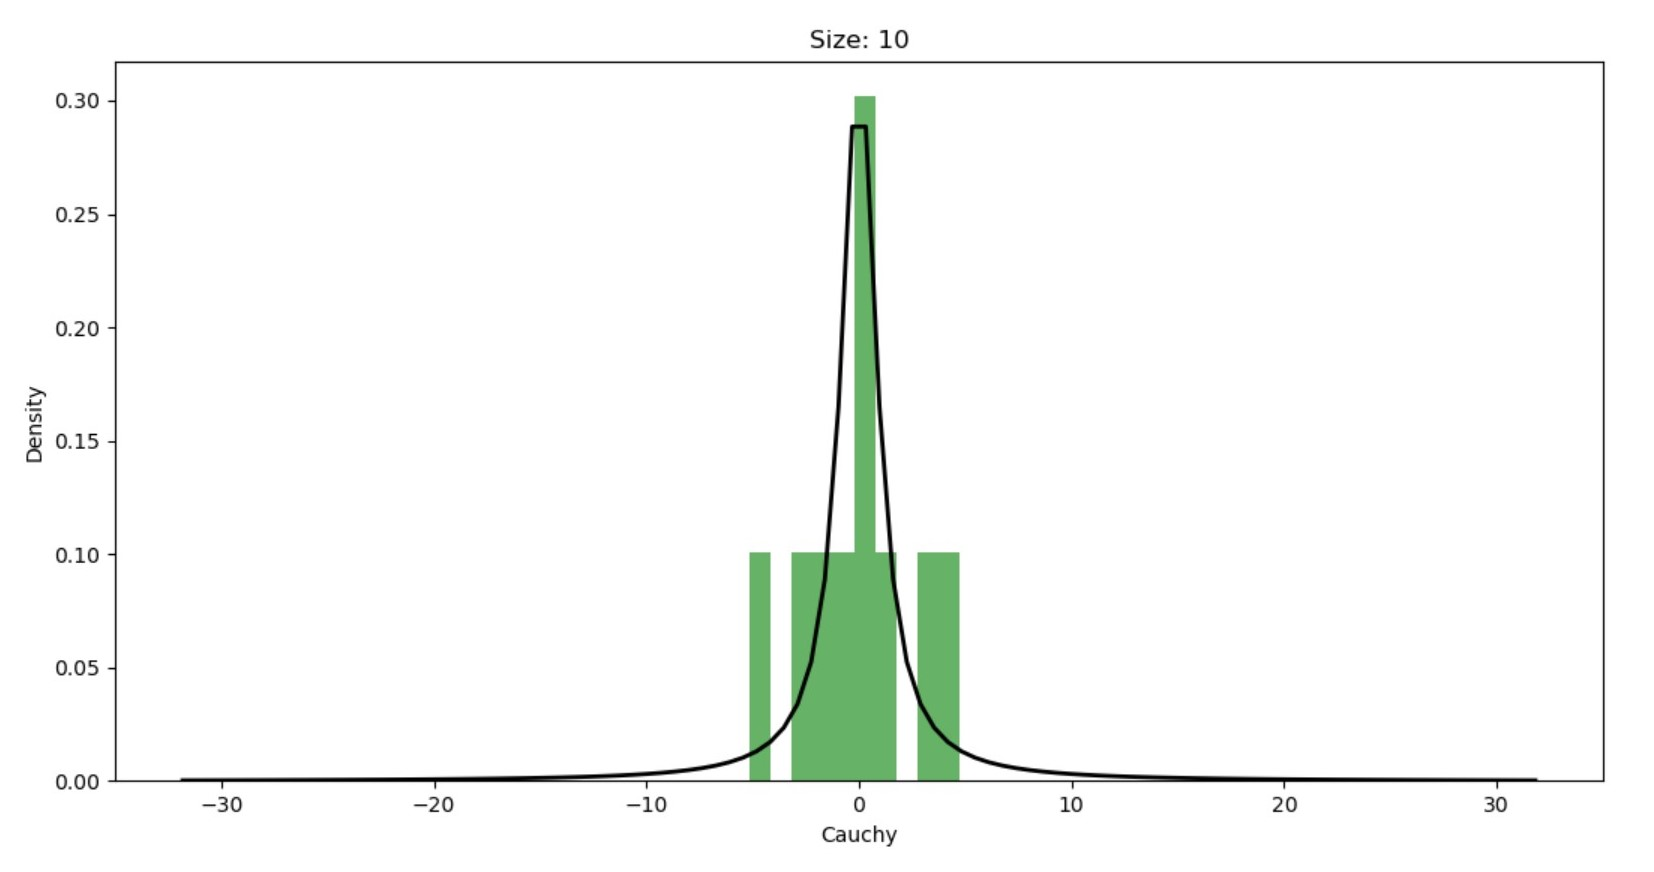
\includegraphics[width=55mm, height =0.25\textheight]{pics/c10.jpg}
			&
			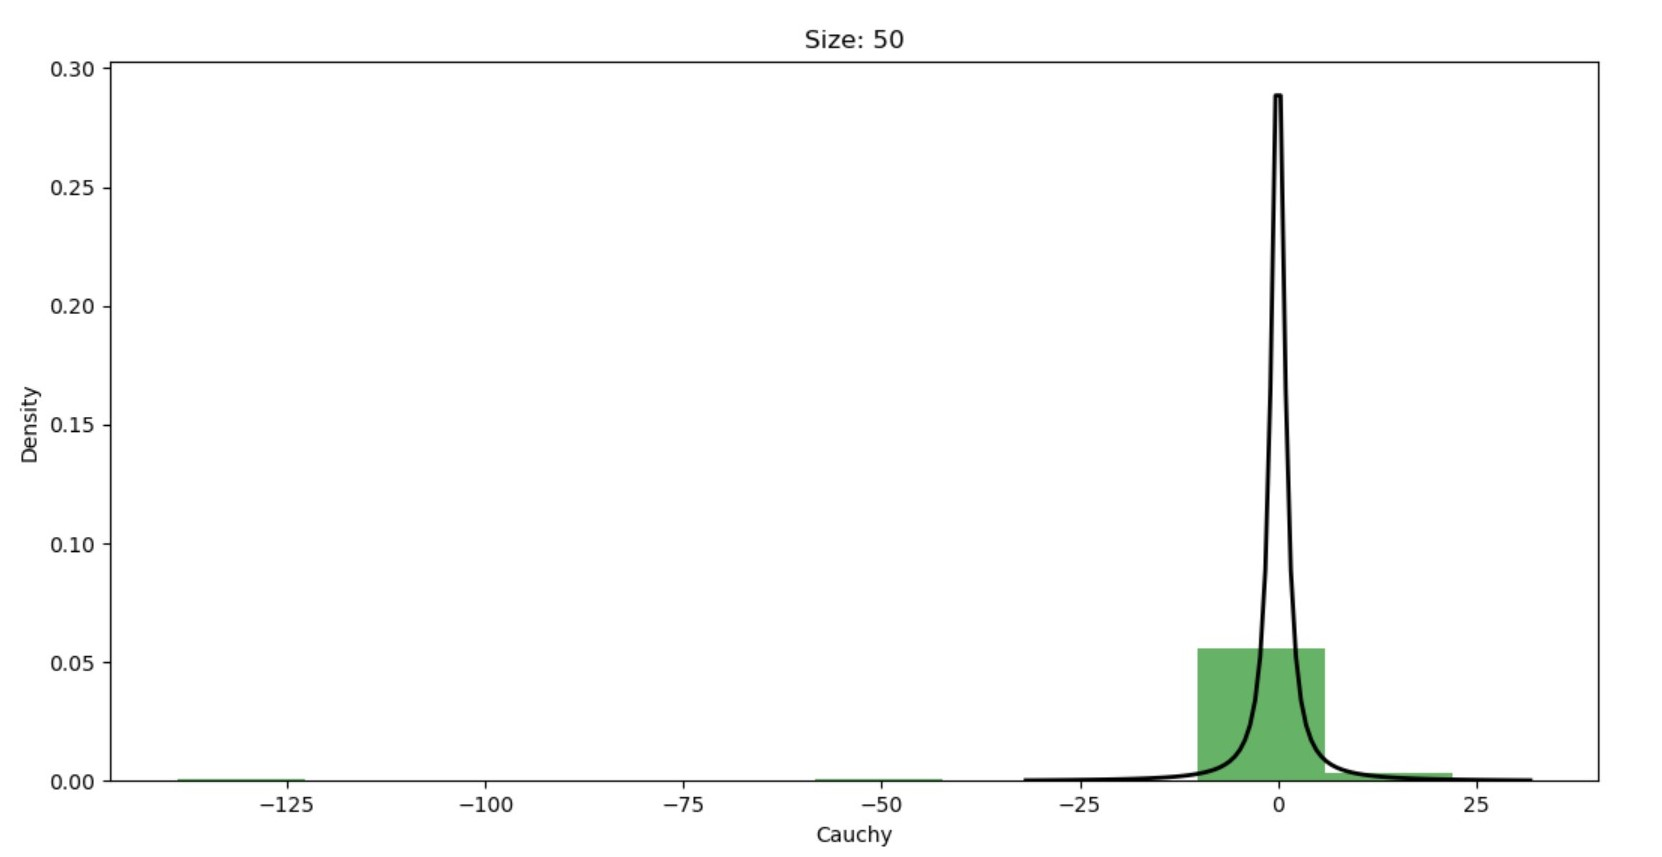
\includegraphics[width=55mm, height =0.25\textheight]{pics/c50.jpg}
			&
			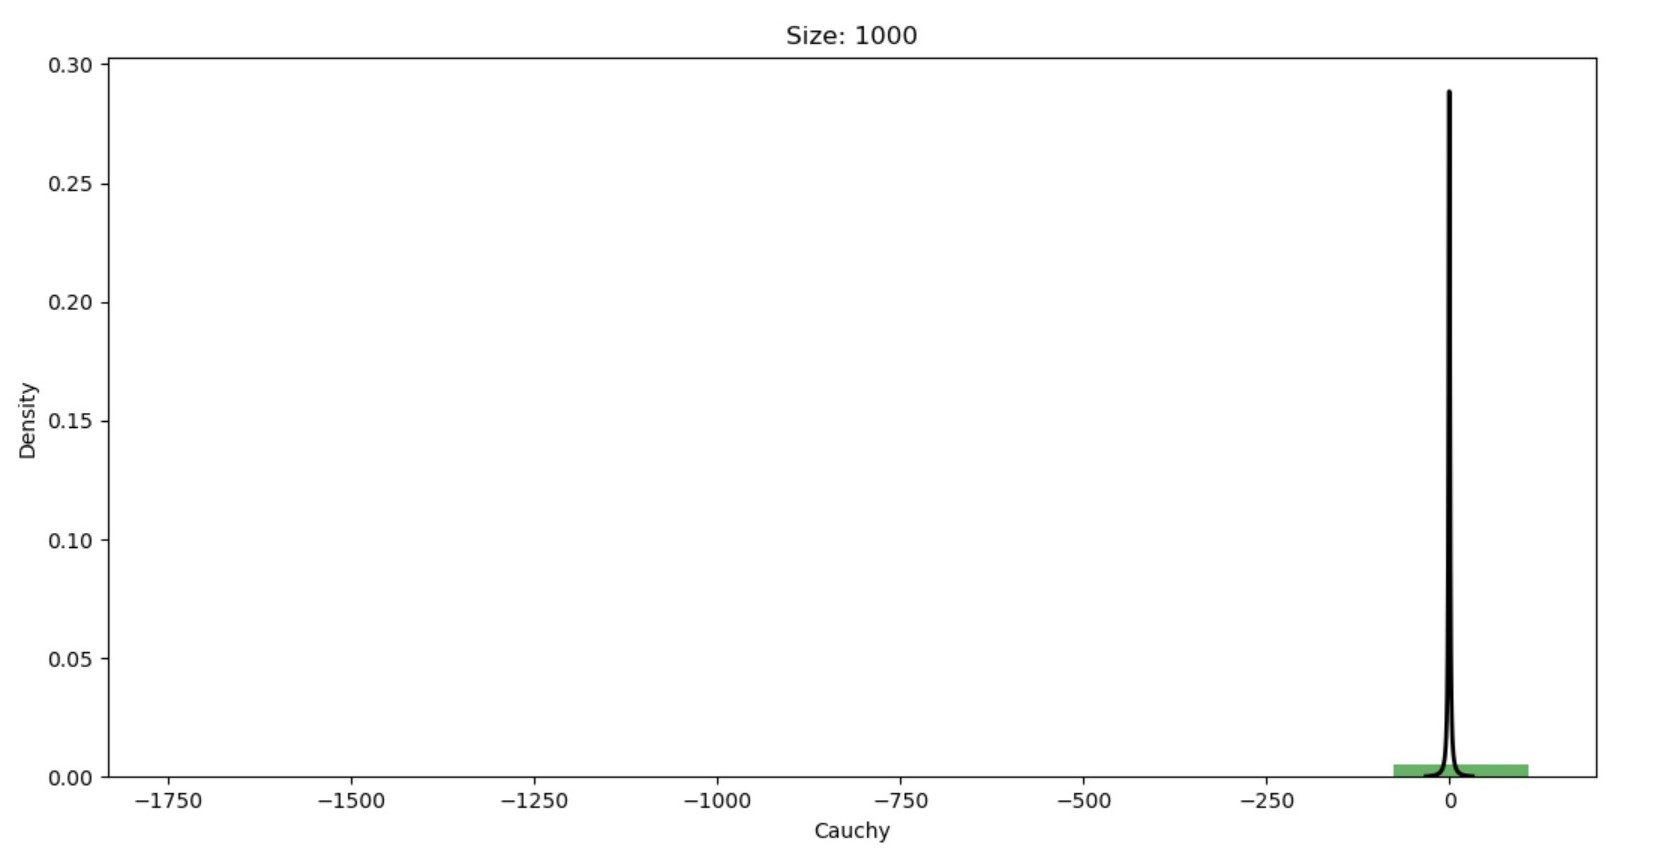
\includegraphics[width=55mm, height =0.25\textheight]{pics/c1000.jpg}
		\end{tabular}
		\caption{Распределение Коши}
		\label{fig:cauchy}
	\end{figure}
	

	\begin{figure}[H]
		\centering
		\begin{tabular}{ccc}
			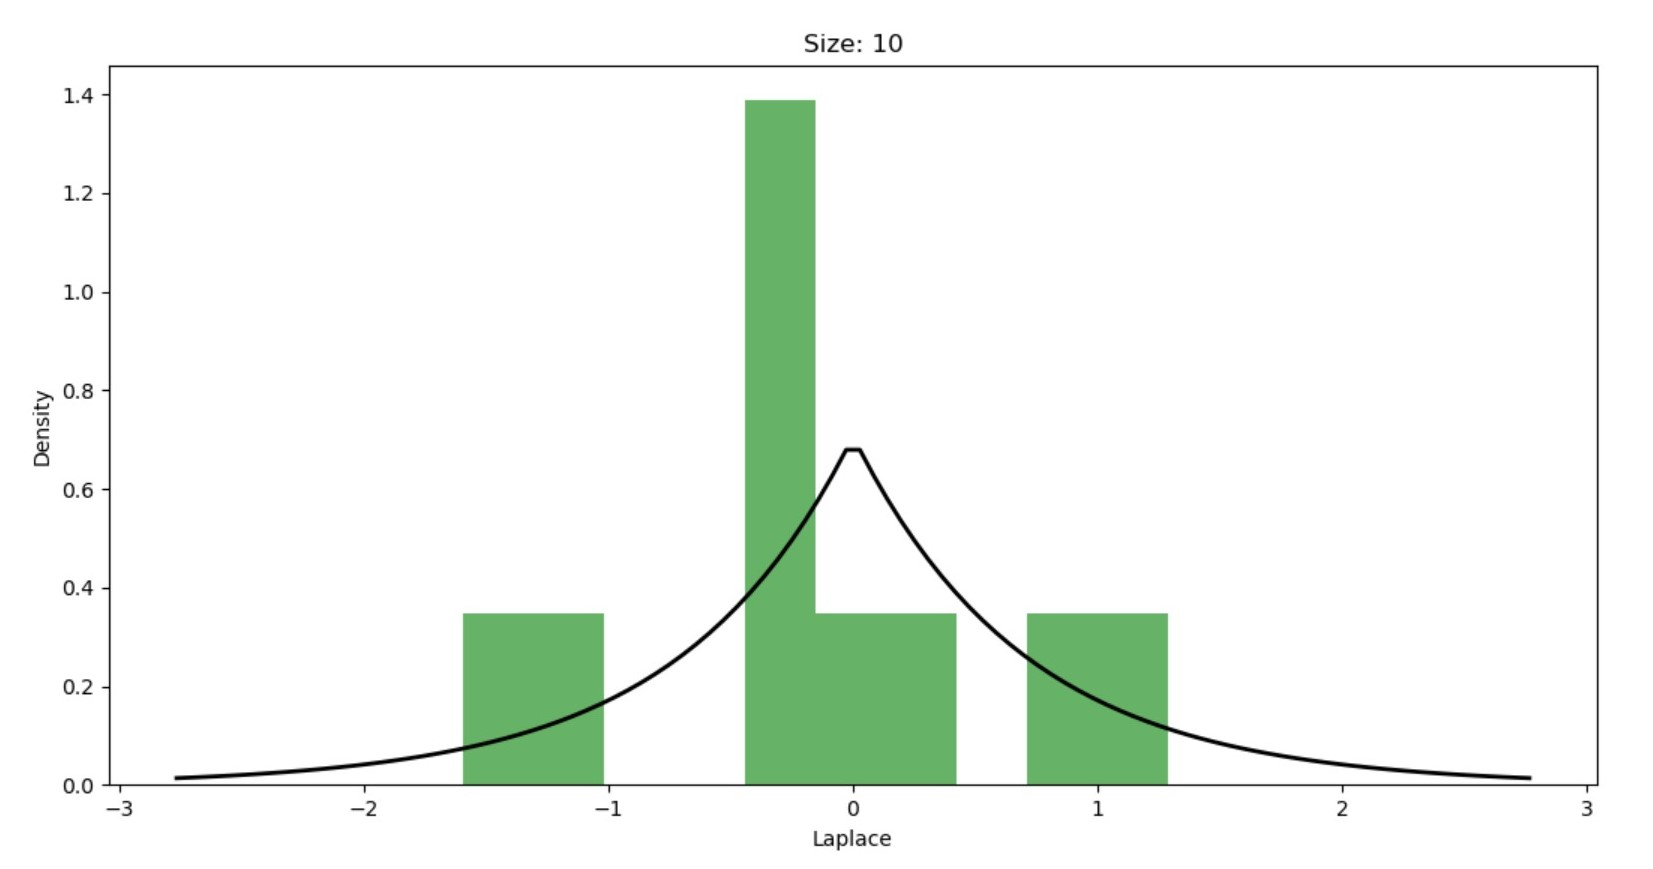
\includegraphics[width=55mm, height =0.25\textheight]{pics/l10.jpg}
			&
			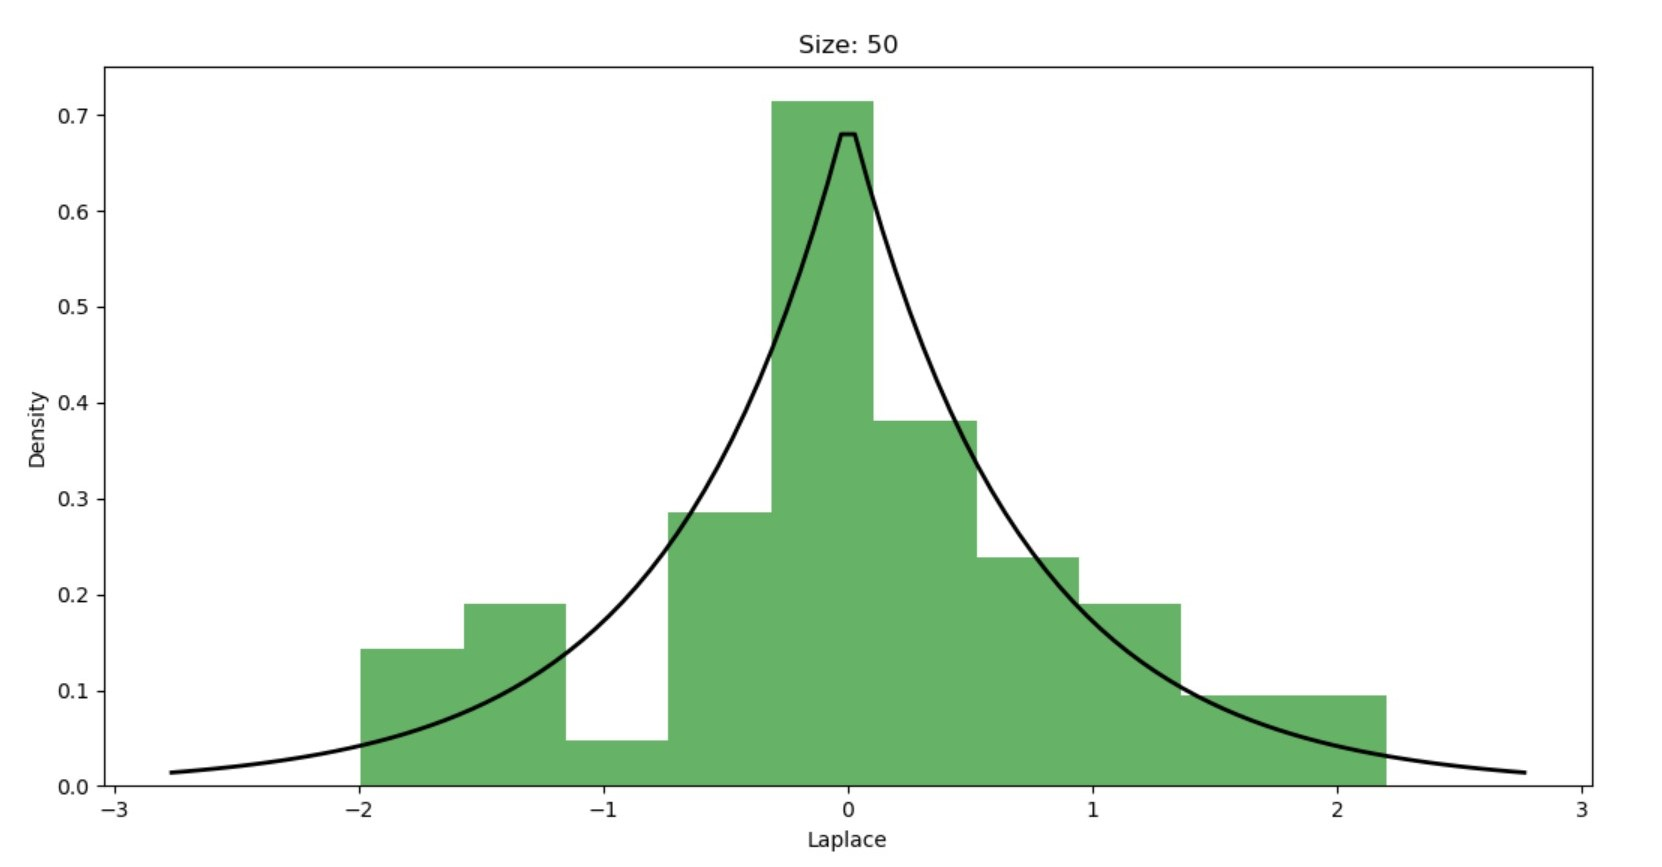
\includegraphics[width=55mm, height =0.25\textheight]{pics/l50.jpg}
			&
			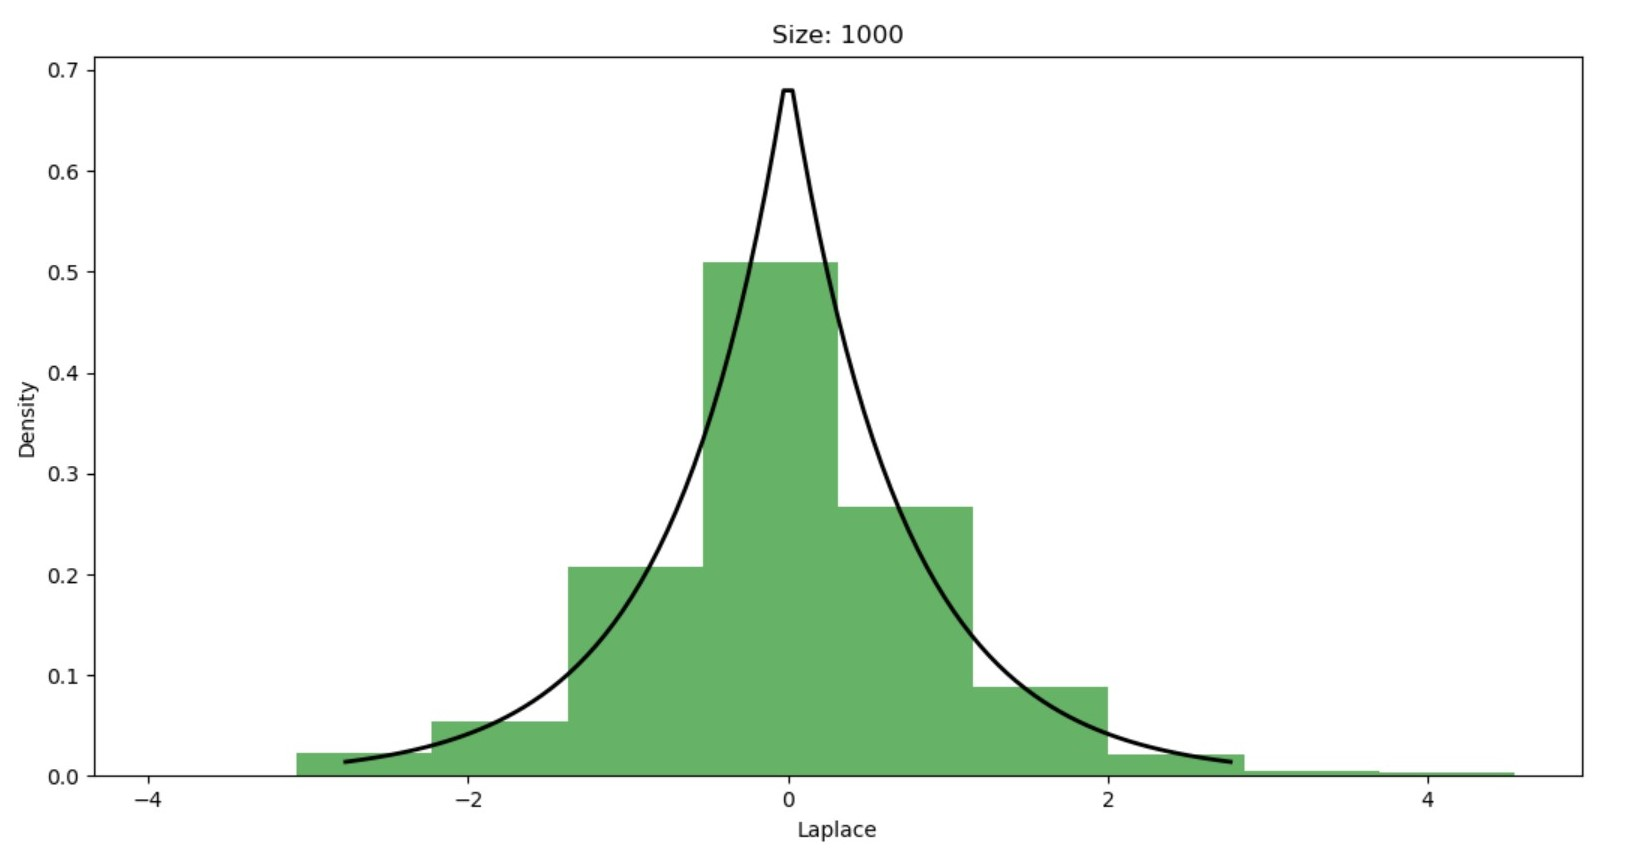
\includegraphics[width=55mm, height =0.25\textheight]{pics/l1000.jpg}
		\end{tabular}
		\caption{Распределение Лапласа}
		\label{fig:laplace}
	\end{figure}


	\begin{figure}[H]
		\centering
		\begin{tabular}{ccc}
			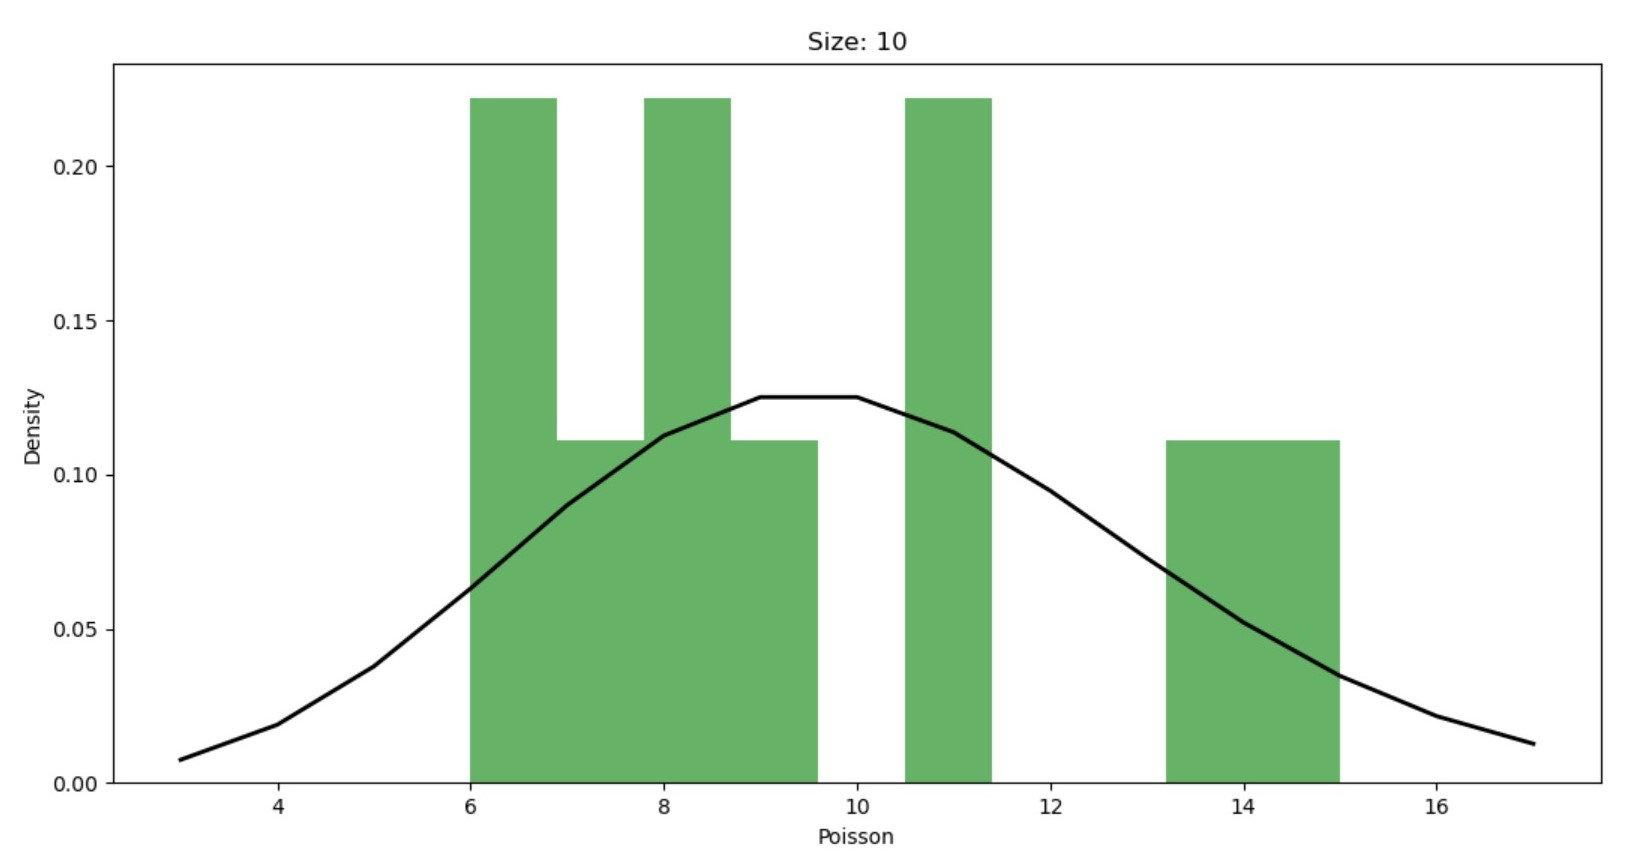
\includegraphics[width=55mm, height =0.25\textheight]{pics/p10.jpg}
			&
			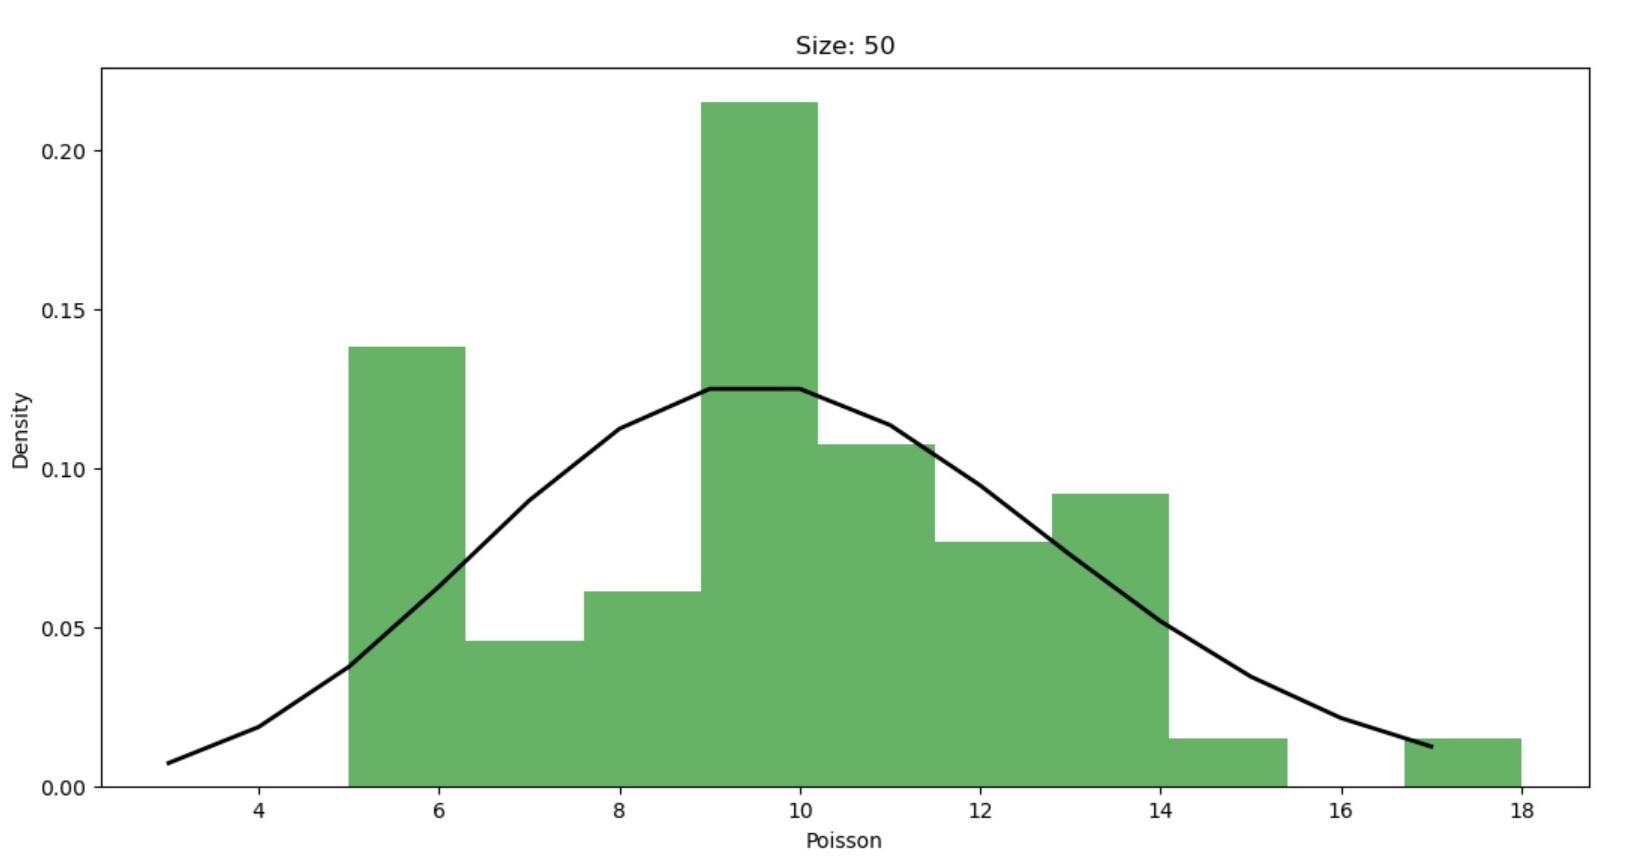
\includegraphics[width=55mm, height =0.25\textheight]{pics/p50.jpg}
			&
			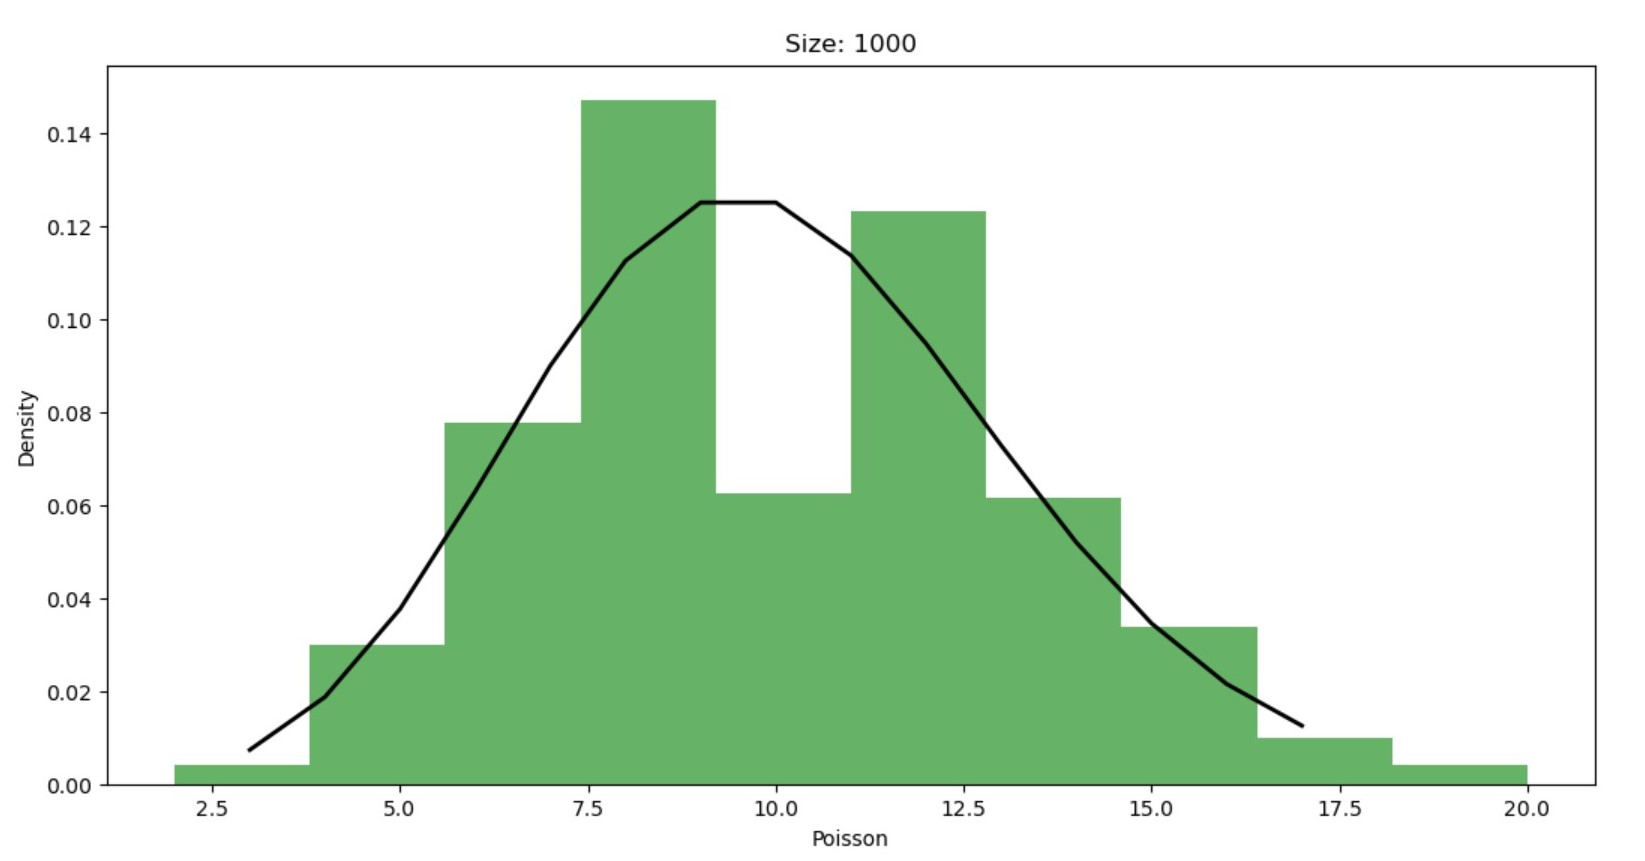
\includegraphics[width=55mm, height =0.25\textheight]{pics/p1000.jpg}
		\end{tabular}
		\caption{Распределение Пуассона}
		\label{fig:poisson}
	\end{figure}


	\begin{figure}[H]
		\centering
		\begin{tabular}{ccc}
			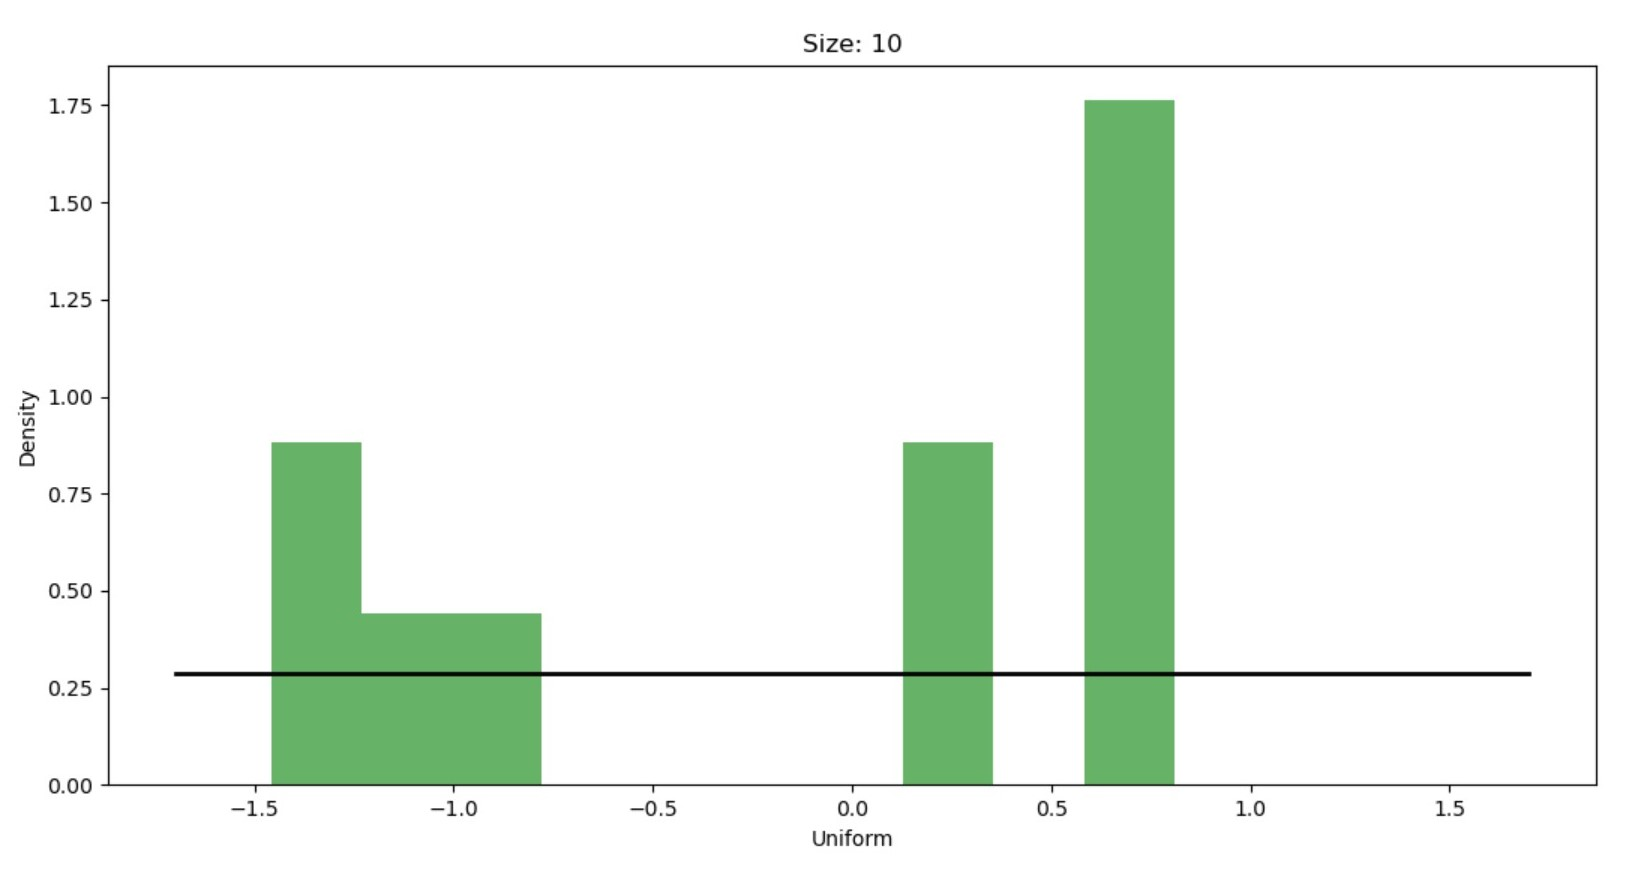
\includegraphics[width=55mm, height =0.25\textheight]{pics/u10.jpg}
			&
			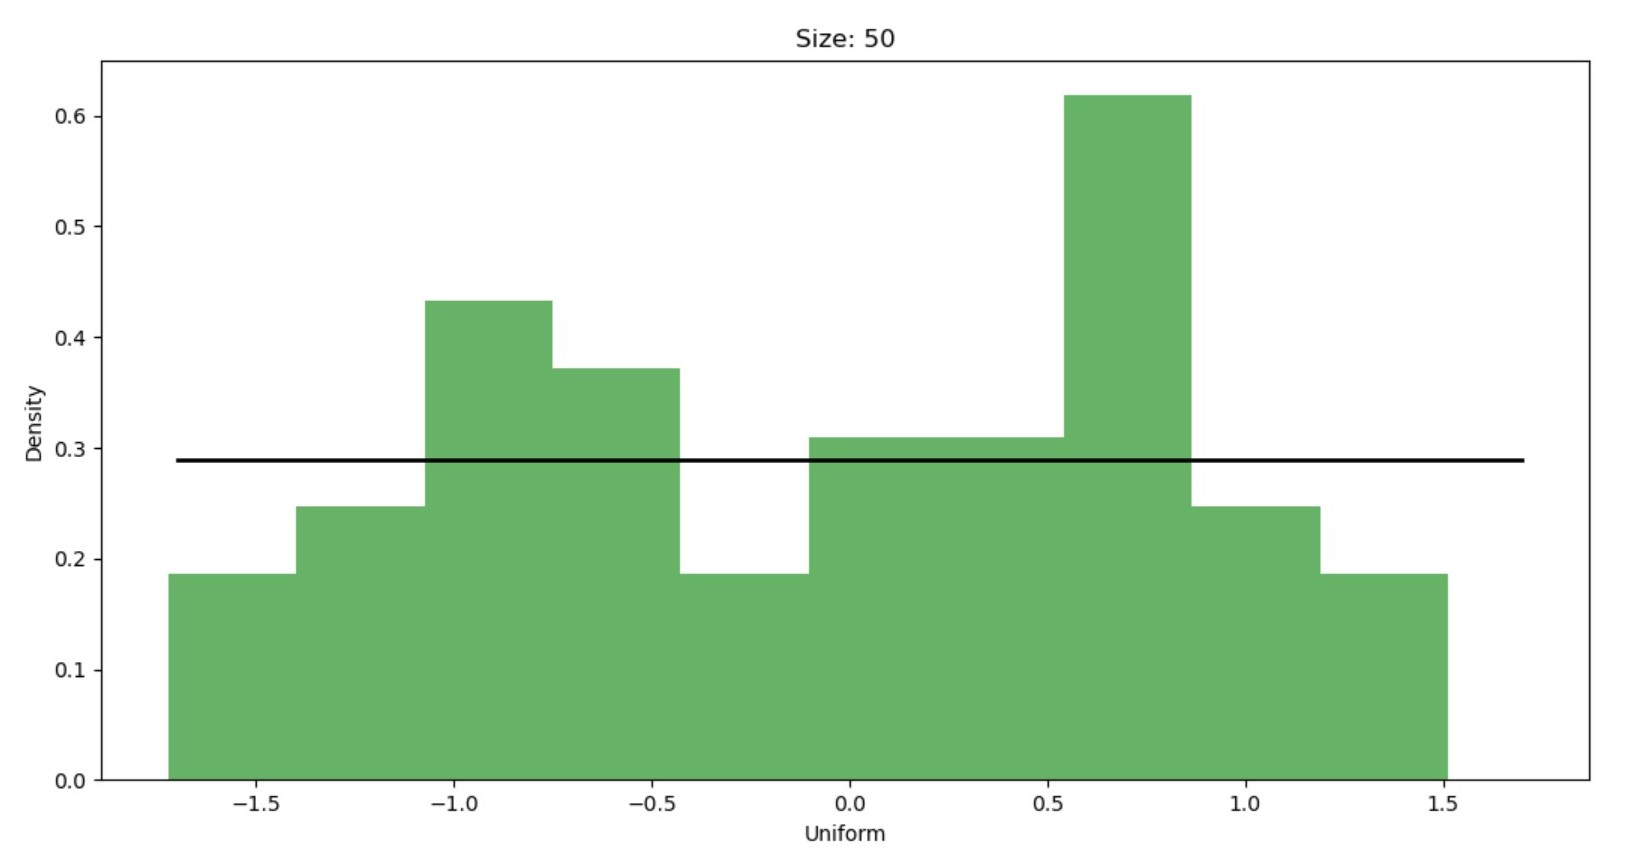
\includegraphics[width=55mm, height =0.25\textheight]{pics/u50.jpg}
			&
			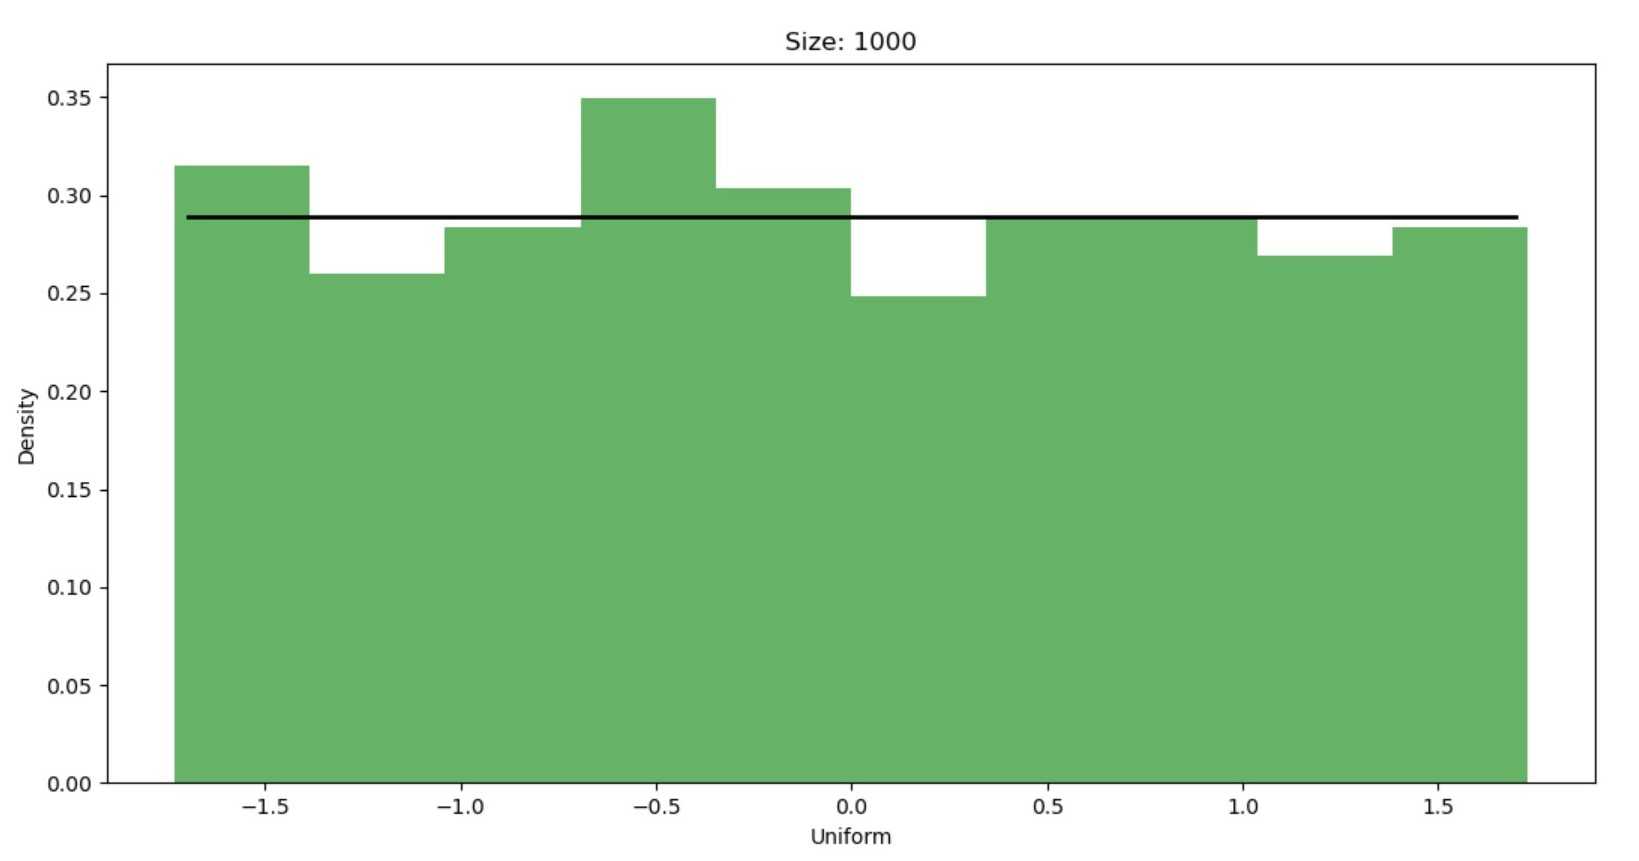
\includegraphics[width=55mm, height =0.25\textheight]{pics/u1000.jpg}
		\end{tabular}
		\caption{Равномерное распределение}
		\label{fig:uniform}
	\end{figure}

\subsection{Характеристики положения и рассеяния}
	\begin{table}[H]
		\centering
		\begin{tabular}[t]{lrrrrr}
			\hline
			Characteristic   &      Mean &    Median &       $z_R$ &      $z_Q$ &      $z_{tr}$ \\
			\hline
			Normal E(z) 10   &  0.025501 &  0.010119 &  0.030651 & 0.030570 &  0.025708 \\
			Normal D(z) 10   &  0.103765 &  0.092774 &  0.476065 & 0.505294 &  0.172139 \\
			Normal E(z) 100  & 0.001106 & 0.001414  &  -0.04678 & 0.008496 & 0.005806 \\
			Normal D(z) 100  &  0.010594 &  0.009886  &  0.461752 & 0.514966 &  0.018883 \\
			Normal E(z) 1000 & -0.000306 & 0.00014  & 0.029287  & 0.017512 & -0.001402 \\
			Normal D(z) 1000 &  0.0010219 &  0.00090 &  0.499531  & 0.498409 &  0.0020510 \\
			\hline
		\end{tabular}
		\caption{Нормальное распределение}
		\label{tab:normal}
	\end{table}

	\begin{table}[ht]
	\centering
		\begin{tabular}[t]{lrrrrr}
			\hline
			Characteristic   &        Mean &    Median &            $z_R$ &       $z_Q$ &      $z_{tr}$ \\
			\hline
			Cauchy E(z) 10   &   -1.82930 &  -0.01278 &   -3.6080     &  -0.6565 &  -1.73308 \\
			Cauchy D(z) 10   &  987.1422    &  0.34462 & 8934.589       &  854.6997 &  1708.300 \\
			Cauchy E(z) 100  &   -8.04716  & -0.002323 & 2.58638      & 3.76963 & -17.4805 \\
			Cauchy D(z) 100  & 90333.65   &  0.024408 &    3996.35 &  5978.85 &  359703.9  \\
			Cauchy E(z) 1000 &   0.0993672  & 0.000122 &  -2.16597     &  -0.68649  & -0.033700 \\
			Cauchy D(z) 1000 & 1228.695   &  0.0024604 &    3185.117 &  1023.5756 &  4370.5033 \\
			\hline
		\end{tabular}
	\caption{Распределение Коши}
	\label{tab:cauchy}
	\end{table}
	
	\begin{table}[ht]
	\centering
		\begin{tabular}[t]{lrrrrr}
			\hline
			Characteristic    &      Mean &    Median &       $z_R$ &       $z_Q$ &      $z_{tr}$ \\
			\hline
			Laplace E(z) 10   &  -0.006466 &  0.000874 & -0.017804 &  -0.029233 &  -0.010286 \\
			Laplace D(z) 10   &  0.0967693 &  0.068329 &  0.529119 &  0.4894004 &  0.159409 \\
			Laplace E(z) 100  & -0.002621 & -0.002186 & 0.0325949 & 0.000488 & -0.007330 \\
			Laplace D(z) 100  &  0.010093 &  0.006105 &  0.5098014 &  0.528626 &  0.020044 \\
			Laplace E(z) 1000 &  -0.000461 &  4.5834-05 &  0.005827 &  0.008741 &  -0.0003342 \\
			Laplace D(z) 1000 &  0.000950 &  0.000526 &  0.503384 &  0.483016 &  0.001967 \\
			\hline
		\end{tabular}
		\caption{Распределение Лапласа}
		\label{tab:laplace}
	\end{table}

	\begin{table}[ht]
		\centering
		\begin{tabular}[t]{lrrrrr}
			\hline
			Characteristic    &      Mean &   Median &       $z_R$ &      $z_Q$ &     $z_{tr}$ \\
			\hline
			Poisson E(z) 10   & 10.0305   & 9.887  	 &  9.9375   & 10.1255  & 10.0543     \\
			Poisson D(z) 10   &  1.05715  & 1.45523  &  5.1613   & 5.0939   & 1.70460  \\
			Poisson E(z) 100  & 9.978119   & 9.8255   & 9.8905   & 9.777 & 9.98496  \\
			Poisson D(z) 100  &  0.097413 & 0.1972  &  5.11775 & 5.105771 & 0.198463 \\
			Poisson E(z) 1000 & 10.00179   & 9.997   & 9.905    & 9.988  & 10.0054 \\
			Poisson D(z) 1000 &  0.009803 & 0.001991 &  5.31547 & 5.15535 & 0.018978 \\
			\hline
		\end{tabular}
		
		\caption{Распределение Пуассона}
		\label{tab:poisson}
	\end{table}

	\begin{table}[ht]
		\centering
		\begin{tabular}[t]{lrrrrr}
			\hline
			Characteristic    &      Mean &    Median &       $z_{R}$ &       $z_Q$ &      $z_{tr}$ \\
			\hline
			Uniform E(z) 10   &  0.017459 &  0.016779 &  0.043340 &  -0.011148 &  0.001145 \\
			Uniform D(z) 10   &  0.098445 &  0.219330 &  0.487425 &  0.5378816 &  0.166308 \\
			Uniform E(z) 100  &  -0.002799 &  -0.00437 &  0.017764 &  0.001040 &  0.002232 \\
			Uniform D(z) 100  &  0.010377 &  0.030492 &  0.443175 &  0.514648 &  0.020929 \\
			Uniform E(z) 1000 & 0.001501 & 0.002397 & -0.033368  & 0.026533 & 0.001575  \\
			Uniform D(z) 1000 &  0.001005 &  0.002988 &  0.5136426   &  0.495917 &  0.002077 \\
			\hline
		\end{tabular}
		\caption{Равномерное распределение}
		\label{tab:uniform}
	\end{table}